\documentclass[10pt,a4paper]{beamer}
\usepackage[utf8]{inputenc}
\usepackage{amsmath}
\usepackage{amsfonts}
\usetheme{Berkeley}
\usepackage{amssymb}
\usepackage{graphicx}
\usepackage{xypic}
\usepackage[all]{xy}
\usepackage{listings}
\lstset{ %
	basicstyle=\footnotesize,
    numbers=left,
    numberstyle=\tiny\color{gray},
    tabsize=10,
}
\author{Richard Torenvliet}
\title{Flood Simulation Browser}
\begin{document}
\begin{frame}
\maketitle
\end{frame}
\begin{frame}
\tableofcontents
\end{frame}
\section{Introductie}
\begin{frame}
\frametitle{Introduction}
\begin{columns}[c]
\column{1.5in}
\begin{itemize}
\item Urban Flood Project
\item Early Warning System
\item Burgers en Hulpdiensten
\item Steeds Belangrijker
\item Sensoren in dijk + Internet
\item Voorlichting met multi-touch table
\item Water Simulatie
\item Hoogte Kaart
\end{itemize}
\column{2.0in}
\begin{figure}
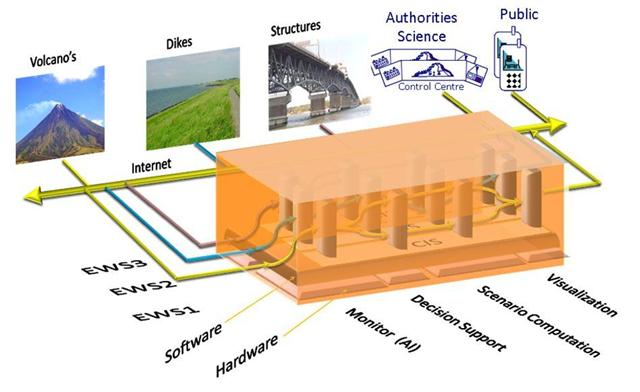
\includegraphics[scale=0.3]{concept.png}
\caption{Bron: \url{http://urbanflood.eu/aboutus.aspx}}
\end{figure}
\end{columns}
\end{frame}
\section{Doel Flood Simulation Browser}
\begin{frame}
\frametitle{Doel Flood Simulation Browser}
\begin{columns}[c]
\column{5cm}
\begin{itemize}
\item Informeren over overstromingsgebied
\item Zien wat er als eerst onderwater gaat
\item Evacuatie routes
\item Hulpdienst routes
\item Browse door alle simulaties
\item Nieuwe simulatie uitvoeren
\end{itemize}
\column{5cm}
\begin{figure}
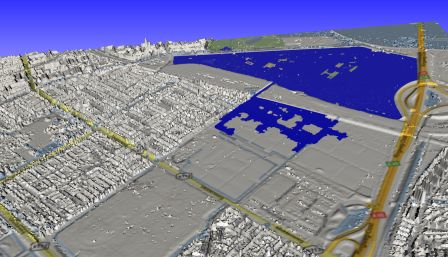
\includegraphics[scale=0.5]{simulation.png}
\caption{Bron: \url{http://urbanflood.eu/default.aspx}}
\end{figure}
\end{columns}
\end{frame}
\section{Dit project}
\begin{frame}
\frametitle{Dit Project}
\begin{itemize}
\item Toegankelijkheid vergroten
\item Browser geschikt maken voor Tablets
\item Server levert plaatjes + coördinaten (Bounding Box)
\item Plaatjes over een kaart leggen, e.g. Google Maps
\item Intuïtief design
\item Extra eis: Crossplatform, daarmee meer publiek
\item Onderzoek taal/framework keuze voor Crossplatform
\item Extra onderzoek: Back-end server testen.
\end{itemize}
\end{frame}
\section{App Design}
\begin{frame}
\frametitle{App Design}
\begin{columns}[c]
\column{5cm}
\begin{itemize}
\item Hoe mensen tablets vasthouden (Clark, 2012)
\item Letten op hierachie bij plaatsing componenten(belangrijke knoppen bovenaan)
\item Weergeven van simulaties (Locaties en bijbehorende simulaties)
\item Simulatiestappen kunnen doorlopen (controls).
\item Plotten van informatie over overstroming.
\end{itemize}
\column{5cm}
\begin{figure}
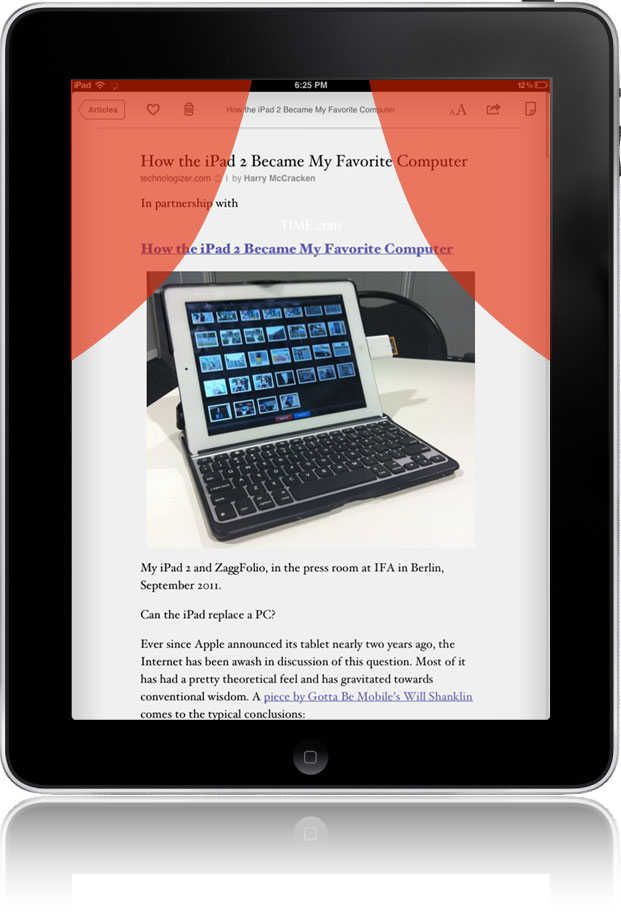
\includegraphics[scale=0.2]{touch.png}
\caption{Bron: \url{} (Clark 2012)}
\end{figure}
\end{columns}
\end{frame}
\section{Platform keuze}
\begin{frame}
\frametitle{Platform keuze}
\begin{itemize}
\item 
	\begin{itemize}
		\item iOS Objective C - niet crossplatform - hoge leercurve
			\item Android Java - idem
		\item jQuery Mobile -  problemen met fixed headers \& footers, combinatie PhoneGap
		\item Titanium - Makkelijk, maar vrij groot, veel geheugen gebruik. Design anders op andere telefoons en niet ECHT crossplatform
	\end{itemize}
\item Sencha Touch 2
\item Voordelen
		\begin{itemize}
		\item Crossplatform
		\item MVC Design Pattern
		\item Mobiele website of App
		\item Android en iOS
		\item Geen PhoneGap nodig
		\end{itemize}
\item Nadelen vooraf
		\begin{itemize}
				\item Verschilde veel met persoonlijke kennis van webtalen
				\item Mogelijk onvoorziene problemen m.b.t. performance
		\end{itemize}
\end{itemize}
\end{frame}
\section{Implementatie}
\begin{frame}
\frametitle{Implementatie}
\begin{columns}
\column{6cm}
\begin{itemize}
\item Sencha Touch 2
\item Download sencha touch + SDK Tools (command line tool)
\item Start met leeg project: \\ \texttt{\$ sencha generate app my\_app}
\item Layouts bieden layout
\item layout: hbox / vbox, Flex 1, 2
\item List Objecten
\item Map Object
\end{itemize}
\column{4cm}
\begin{figure}
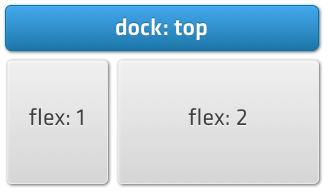
\includegraphics[scale=0.3]{docktop.png}
\end{figure}
\begin{figure}
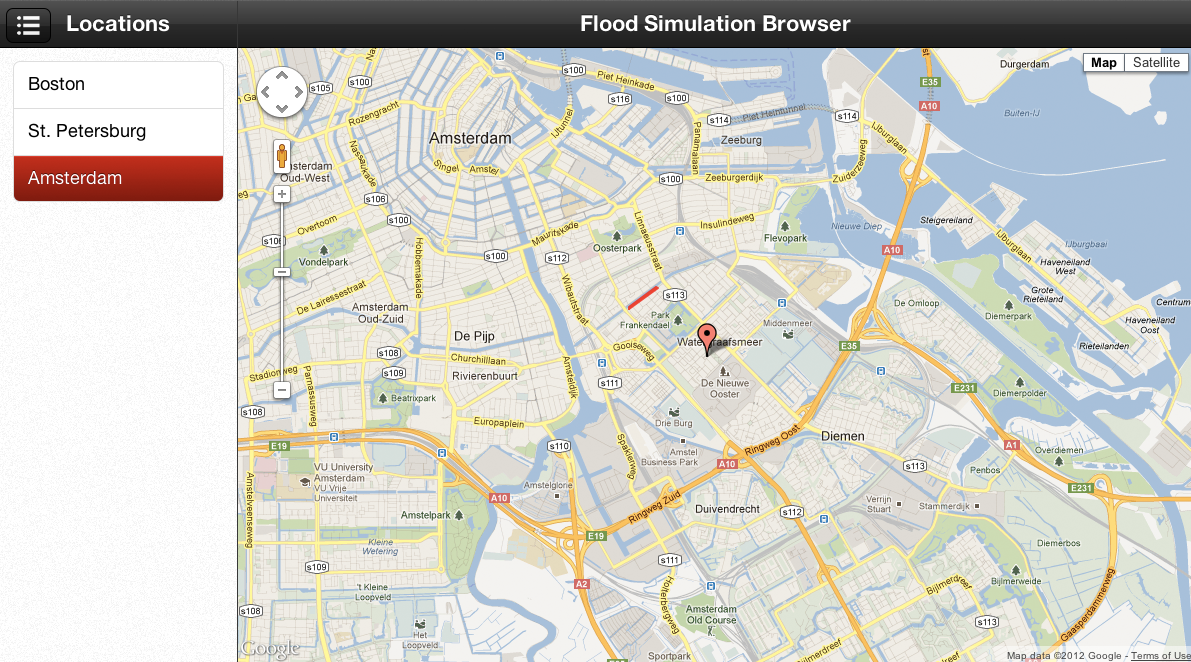
\includegraphics[width=4cm]{ui/fsb_layout.png}
\end{figure}
\end{columns}
\end{frame}
\begin{frame}
\begin{itemize}
\item List \& Stores
\end{itemize}
\begin{figure}[h!]
\xymatrix{
  *+<5ex>[F]{Store}\ar[r]^{\txt<5pc>{fields}} &   *+<5ex>[F]{List}\ar[r] & 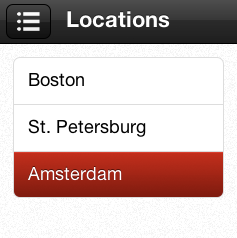
\includegraphics[scale=0.2]{ui/citieslist.png}\ar[dr] \\
  *+<5ex>[F]{Store}\ar[r]^{\txt<5pc>{fields}} &   *+<5ex>[F]{List}\ar[rr] & & 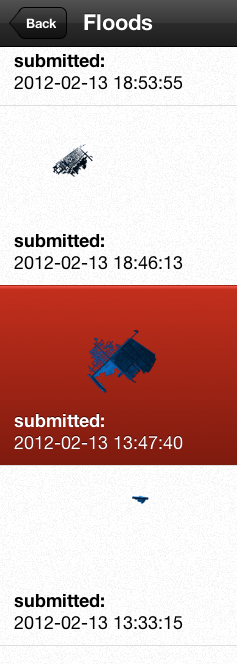
\includegraphics[scale=0.2]{ui/simselected.png}
}
\caption{Stores and Lists}
\end{figure}
\end{frame}
\begin{frame}
\frametitle{Simulatie}
\begin{itemize}
\item Start simulatie
\item Controls, \\
        next step, prev step, play forward, play backwards
\item Tap \& Drag
\end{itemize}
\begin{figure}
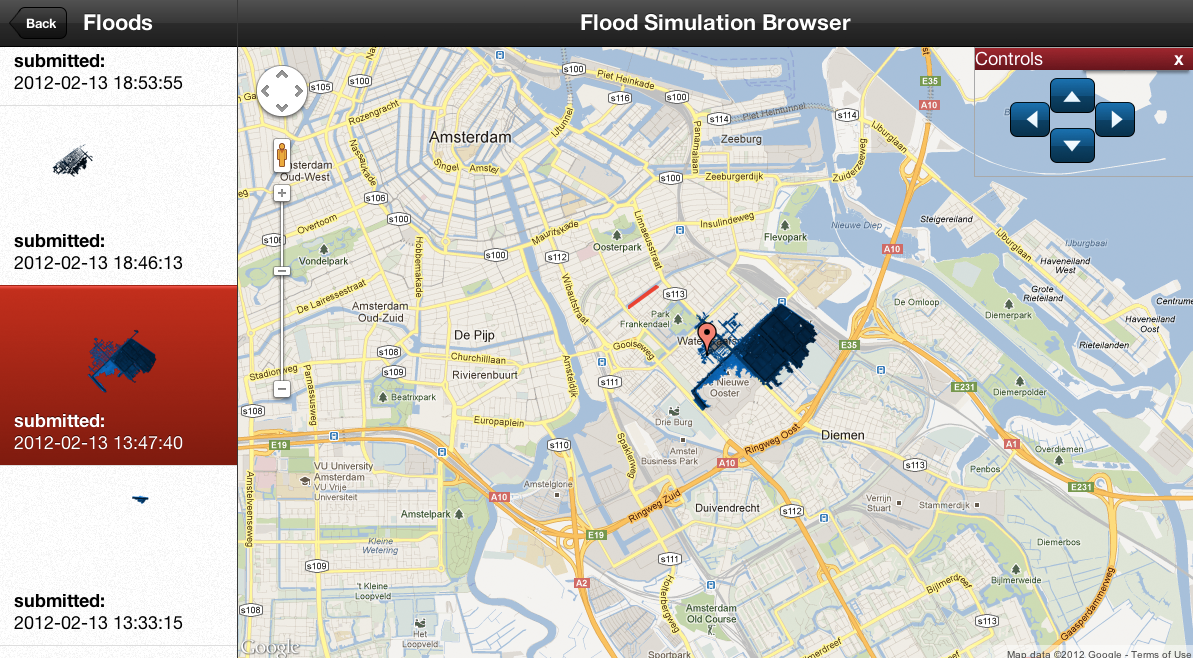
\includegraphics[scale=0.2]{ui/simselected_full.png}
\end{figure}
\end{frame}
\begin{frame}
\begin{itemize}
\frametitle{Volume Chart}
\item Tap op de kaart
\item Volume informatie van dichtsbijzijnde locatie van tap
\item Tap \& Drag
\end{itemize}
\begin{figure}
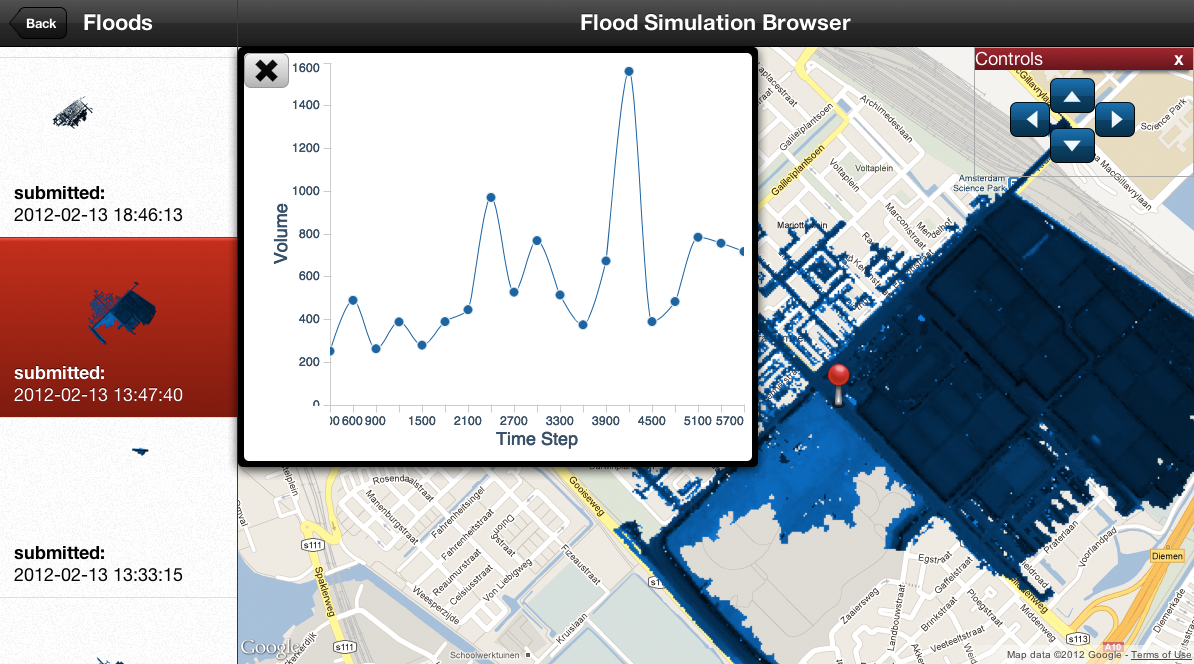
\includegraphics[scale=0.2]{ui/floodchart.png}
\end{figure}
\end{frame}
\begin{frame}
\begin{itemize}
\frametitle{Simulatie Mensen}
\item Selecteer simulatie Lsm
\item Tap locatie, tap simulatie
\end{itemize}
\begin{figure}
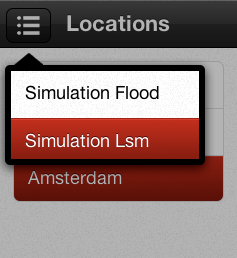
\includegraphics[scale=0.2]{ui/select_lsm.png}
\end{figure}
\begin{figure}
	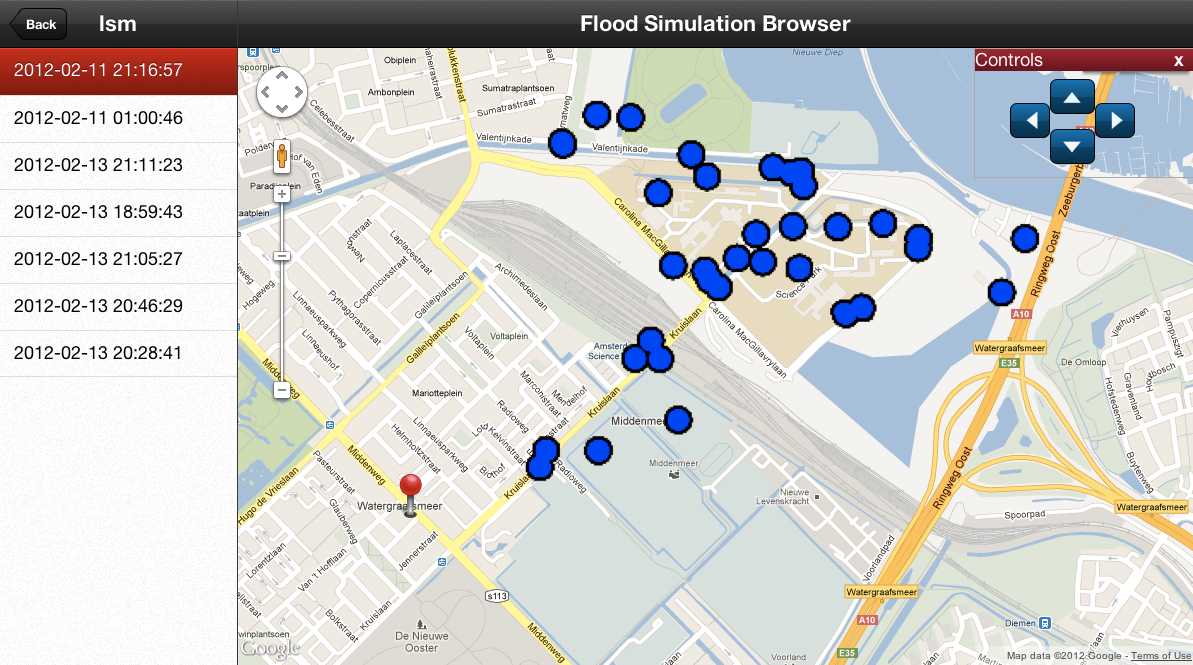
\includegraphics[scale=0.2]{ui/lsm.png}
	\caption{lsm}
\end{figure}
\end{frame}
\begin{frame}
\begin{itemize}
\frametitle{Deployment}
\item Snel testen in browser (webkit)
\item Build naar device:\texttt{\$ sencha app build native}
\item \texttt{packager.json}
\begin{itemize}
	\item iOSSimulator
	\item iOS
	\item Android
	\item AndroidEmulator
\end{itemize}
\end{itemize}
\end{frame}

\section{Server Testing}
\begin{frame}[fragile]
\frametitle{Test in Browser}
\begin{itemize}
\item Tool: Siege
\item Server: \url{sangkil.science.uva.nl} (E5620 Xeon Duo @2.4 Ghz, 32 GB Ram)
\item Bottle necks vermijden: \url{mangkus.science.uva.nl}
\item Praktisch naast elkaar
\item file met verschillende requests, random uitgevoerd
\item Concurrente processen
\item Herhalingen
\end{itemize}
\begin{lstlisting}
#!/bin/bash
rep=(10 50 100 200 300 400 500)
for i in "${rep[@]}"
do
	siege -i -b -f /path/to/requests_file.txt -c $i -r $1
done
\end{lstlisting}
\end{frame}
\begin{frame}
\begin{figure}
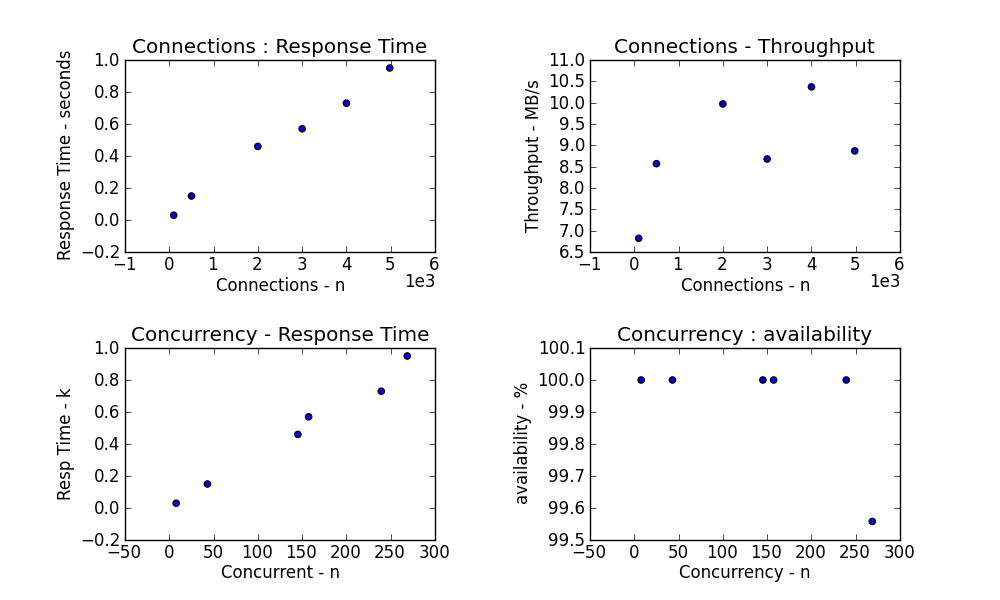
\includegraphics[scale=0.4]{siege_10r.png}
%siege_100r.log.png
%siege_200r.log.png}
\caption{10 repetities, getest: 10 50 200 300 400 500 concurrent}
\end{figure}
\end{frame}
\begin{frame}
\begin{figure}
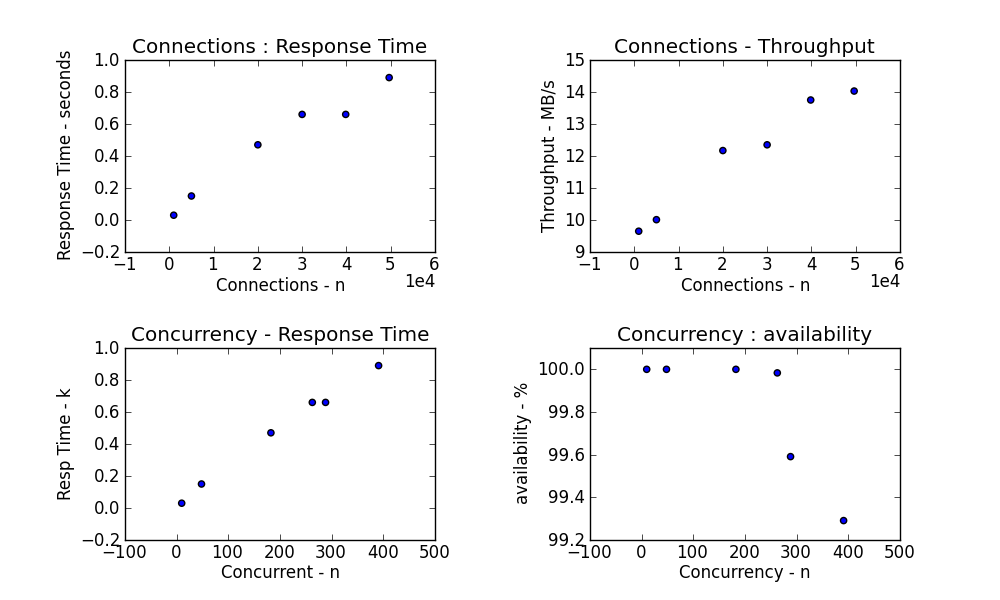
\includegraphics[scale=0.4]{siege_100r.png}
%siege_100r.log.png
%siege_200r.log.png}
\caption{100 repetities, test: 10 50 200 300 400 500 concurrent}
\end{figure}
\end{frame}

\begin{frame}
\begin{figure}
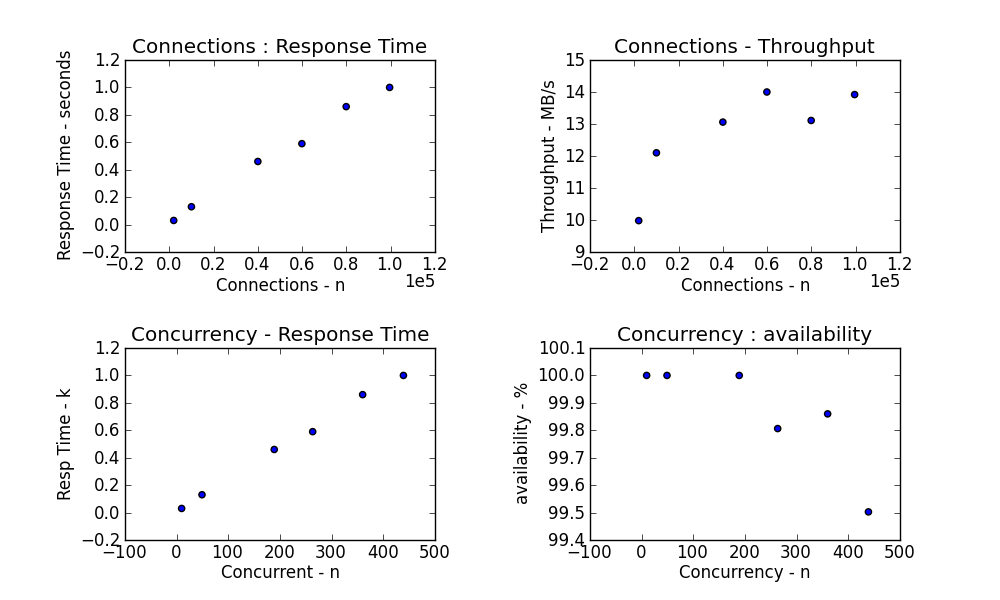
\includegraphics[scale=0.4]{siege_200r.png}
%siege_100r.log.png
%siege_200r.log.png}
\caption{200 repetities, getest: 10 50 200 300 400 500 concurrent}
\end{figure}
\end{frame}

\section{Referenties}
\begin{frame}
\begin{thebibliography}{9}
\frametitle{Referenties}
\bibitem{urban flood}
  Urban Flood Project,
  \url{http://urbanflood.eu/default.aspx}.

\bibitem{Sencha Touch}
	Sencha Touch 2.
	\url{http://docs.sencha.com/touch/2-0/}.

\bibitem{Google Maps API}
	Google Maps API,
	\url{https://developers.google.com/maps/}.
\bibitem{PhoneGap}
	PhoneGap
	\url{http://www.PhoneGap.com}.
\bibitem{Titanium Mobile}
	Titanium Appcelerator,
	\url{http://www.appcelerator.com/}.
\bibitem{Scalability}
	Freimuth, D., Hu E.,LaVoie,  J.,Mraz, R., Nahum, E., Pradhan, P., \& Tracey, J. (2005). Server Network Scalability and TCP Offload.
	IBM T. J. Watson Research Center
\bibitem{Touch}
	Clark,  J.(2012). designing-touch. \url{http://www.netmagazine.com/features/designing-touch}.
\end{thebibliography}
\end{frame}
\begin{frame}
\bibliographystyle{plain}
\bibliography{references}
\end{frame}
\end{document}